\chapter{Preliminary concepts}

\section{Dynamical Systems}

[introducir bien el tema]. 

The general form for a dynamical system is the following.

\begin{equation}
    \dfrac{d\bm{u}}{dt} = \bm{f}(\bm{u}, \eta), \qquad \bm{f} : \mathbb{R}^N \times \mathbb{R}^{n_\eta} \to \mathbb{R}^N
    \label{eq:def_ds}
\end{equation}

Here, $\bm{u}$ represents the state vector of the system, it might correspond to the
concentrations of different chemicals, the population of certain species or the amplitude
of an electric field. The temporal evolution of the state of the system is thus determined by 
the vector function $\bm{f}$. This function may, in turn, depend on one or more control
parameters $\eta$ relevant to the modeled experiment (i.e. driving frequency, pumping power, etc).

In this thesis, different dynamical systems in the form of Eq.~(\ref{eq:def_ds}) with a {\em nonlinear} function
$\bm{f}$ will be considered. Although it might be argued that, at a fundamental level, the physical laws
that describe the evolution of a system are linear (such as the Schrödinger equation), when one looks at meso- or macroscopical
systems, nonlinear terms naturally arise due to the coarse-graining of the microscopical degrees of freedom [ref Karadr].


In the case of a nonlinear dynamical system, it becomes extremely difficult, and often impossible, to find
general explicit solutions of Eq.~(\ref{eq:def_ds}). But it turns out that in most cases, an in-depth
description of the model can be provided by studying only the steady states ($\bm{f}(\bm{u}, \eta) = 0$) and their qualitative changes as parameters 
are varied. In other words, the problem can be reduced to finding the {\em equilibria} and {\em bifurcations} of the system.
In the following section, the elementary bifurcations a system can experience will be described.

\section{Bifurcations}

Qualitative changes of equilibria as parameters are varied.

% Ideas:
% \begin{enumerate}
%     \item saddle-node for genes pp 249
%     \item magnetism Landau Pitchfork
%     \item Hopf, van der pol, bici
% \end{enumerate}

\subsection{Saddle-Node bifurcation}

{\em Saddle-node} or {\em fold} bifurcations provide the simplest mechanism 
for which a pair of stable and unstable equilibria can be created (or destroyed) 
as the control parameter is changed. Although they arise in a huge variety of systems 
[insert ref], close to the bifurcation point the dynamics can always be reduced to
the following minimal or {\em normal form}.

\begin{equation}
    \dfrac{du}{dt} = \eta - u^2
    \label{eq:pre_bif_sn}
\end{equation}

Following the notation of Eq.~(\ref{eq:def_ds}), u represents the state variable
and $\eta$ the control parameter. For $\eta > 0$, the system presents two equilibria $u_{\pm} = \pm\sqrt{\eta}$, where $u_+$ is
stable and $u_-$ unstable. An interesting case occurs when $\eta = 0$, at which point $u = 0$ is
half-stable (stable for positive perturbations and unstable for negative perturbations). Lastly,
for $\eta < 0$ there are no equilibria. Figure~(\ref{fig:pre_bifs_sn}) provides a visual representation
of the previous analysis.

In short, as the bifurcation parameter $\eta$ is decreased (increased)
starting from positive (negative) values, the two equilibria attract (repel) each other and suddenly annihilate (appear).

\begin{figure}[h]
    \centering
    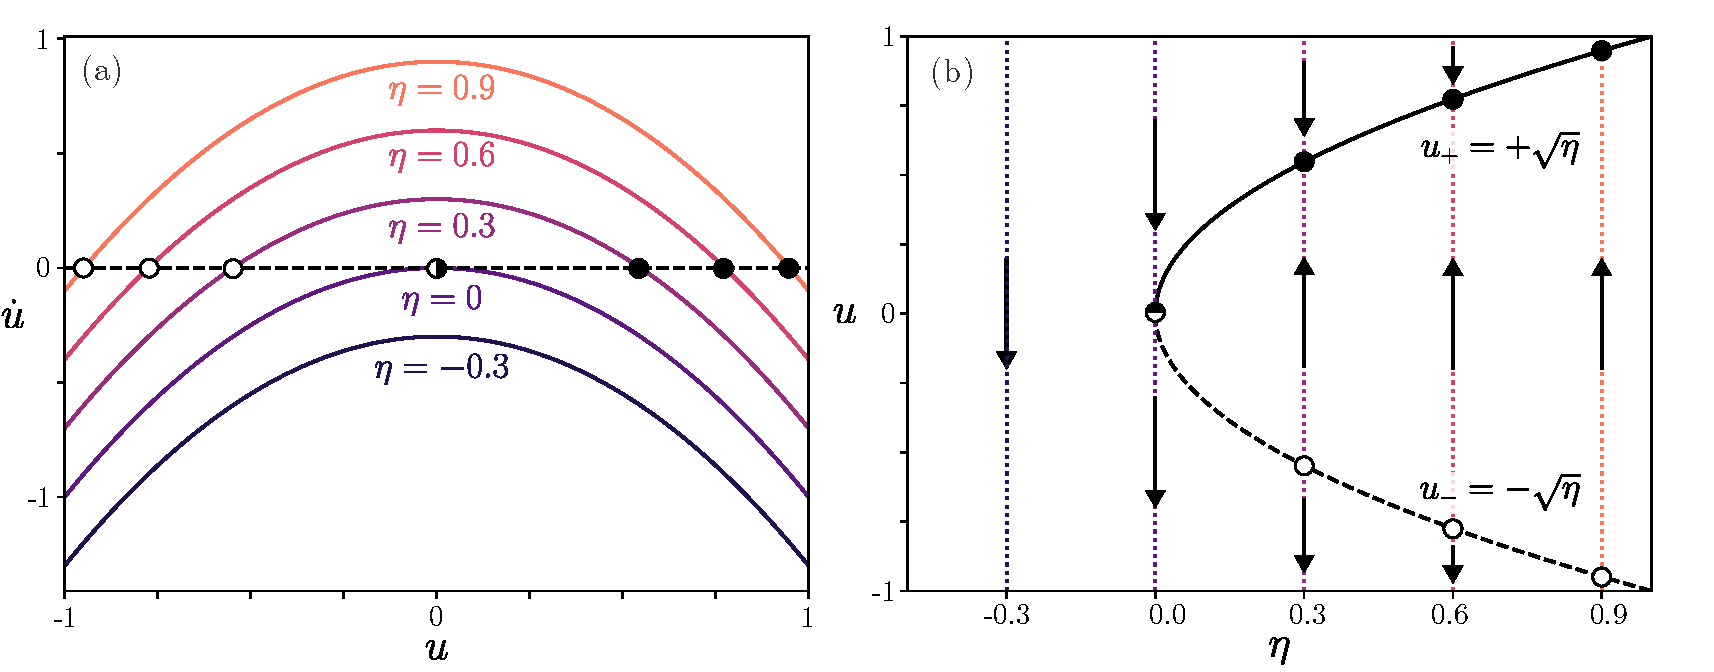
\includegraphics[width=\textwidth]{imagenes/framework/bif_sn_f.pdf}
    \caption{Prototipical scenario for a saddle-node bifurcation. (a) Phase space
    showing both stable and unstable fixed points for different values of $\eta$. 
    Black (white) circles represent
    stable (unstable) fixed points. (b) Bifurcation diagram showing
    the creation of a stable-unstable pair of fixed points. Solid (dashed) line represents
    stable (unstable) branch.}
    \label{fig:pre_bifs_sn}
\end{figure}

\begin{exmp}
    For centuries, the mystery of synchronization between fireflies has
    captivated many people. Although many open questions remain on this topic [ref],
    we will aim to shed {\em light} on this topic only with the knowledge of saddle-node bifurcations
    and a simple model proposed by Ermentrout and ...[ref]. 
    
    Consider the problem
    of a firefly flashing under the presence of a periodically flashing light.
    We will model the flashing of the firefly with an angular variable $\theta$
    such that $\theta = 0$ represents the firefly's flash. The firefly has its 
    own inherent frequency $\omega$, i.e. in the absence of stimuli 
    $\dot{\theta} = \omega$. On the other hand, the periodic stimulus will be
    represented by a phase $\phi$ that satisfies $\dot{\phi} = \Omega$, where 
    $\Omega$ is of course the stimuli period. In order to synchronize with the
    stimuli, the firefly will either want to speed up if it is lagging behind
    or slow down if it is going too fast. The simplest non-linear model that
    fulfills these assumptions is the following,
    \begin{align*}
        \dot{\phi} &= \Omega \\
        \dot{\theta} &= \omega + A \sin(\phi -  \theta)
    \end{align*}

    Subtracting both equations and defining $\varphi = \dot{\phi} - \dot{\theta}$
    yields 

    \begin{equation*}
        \dot{\varphi} = \Omega - \omega - A \sin \varphi
    \end{equation*}

    which can be adimensionalized by rescaling $t \to At$ and introducing
    the non-dimensional parameter $\mu = (\Omega - \omega)/A$,

    \begin{equation}
        \dot{\varphi} = \mu - \sin \varphi
        \label{eq:pre_bif_sn_exmp}
    \end{equation}

    For $\mu = 0$ where the forcing and intrinsic frequencies are the same, there
    is a stable fixed point at $\varphi = 0$ and an unstable fixed point at $\varphi = \pi$.
    As $\mu$ increases, both equilibria approach each other until they collide for $\mu=\mu_c=1$
    at $\varphi = \pi/2$
    and then disappear for $\mu > 1$. We can recognize that the pair of fixed
    points appear (or disappear) through a saddle-node bifurcation.
    
    Moreover, close to the bifurcation point where $\mu_c = 1$ and $\varphi_c = \pi/2$,
    we can do a Taylor expansion: $\mu = 1 + \eta$ and $\varphi = \pi/2 + u$ 
    where $\eta, u \ll 1$. Using the identity $\sin \varphi = \sin (\pi/2 + u) = \cos u$
    and inserting the previous ansatz into Eq.~(\ref{eq:pre_bif_sn_exmp}) yields
    the following
    \begin{align*}
        \dot{\varphi} = \dot{u} &= 1 + \eta - \cos u \\ 
        &\approx 1 + \eta - (1 - \dfrac12 u^2) \\
        &= \eta - \dfrac12 u^2
    \end{align*}

    Which after adequate rescaling corresponds exactly with the saddle-node
    normal form.
    

\end{exmp}

\subsection{Pitchfork bifurcation}

{\em Pitchfork} bifurcations typically arise in systems with symmetry and 
provide a universal mechanism for symmetry-breaking [ref strogatz]. 
A simple example is given by the statistical description of magnetization. 
In the absence of an external field, the net magnetization $m$ 
(below the critical temperature $T_c$) can either be positive or negative 
with no preferred orientation, thus depending only on the initial condition. On the
other hand, if the system is heated above the critical temperature, no net magnetization
is observed, i.e. $m=0$. In the context of statistical mechanics, this second-order
transition can be described by a mean-field approximation from Landau theory, where
the free energy functional is expanded in (even) powers of $m$, thus arriving at exactly
the pitchfork normal form, given by

\begin{equation}
    \dfrac{du}{dt} = \eta u - u ^ 3.
    \label{eq:pre_bif_pitchfork}
\end{equation}

As shown in Fig.~(\ref{fig:pre_bif_pitchfork}), for $\eta < 0$ there is only one 
equilibrium of Eq.~(\ref{eq:pre_bif_pitchfork}), it is stable and corresponds
to the trivial solution $u=0$. For $\eta > 0$, the trivial solution loses stability
and two stable symmetric branches $u_\pm = \pm \sqrt{\eta}$ emerge. 

\begin{figure}[h]
    \centering
    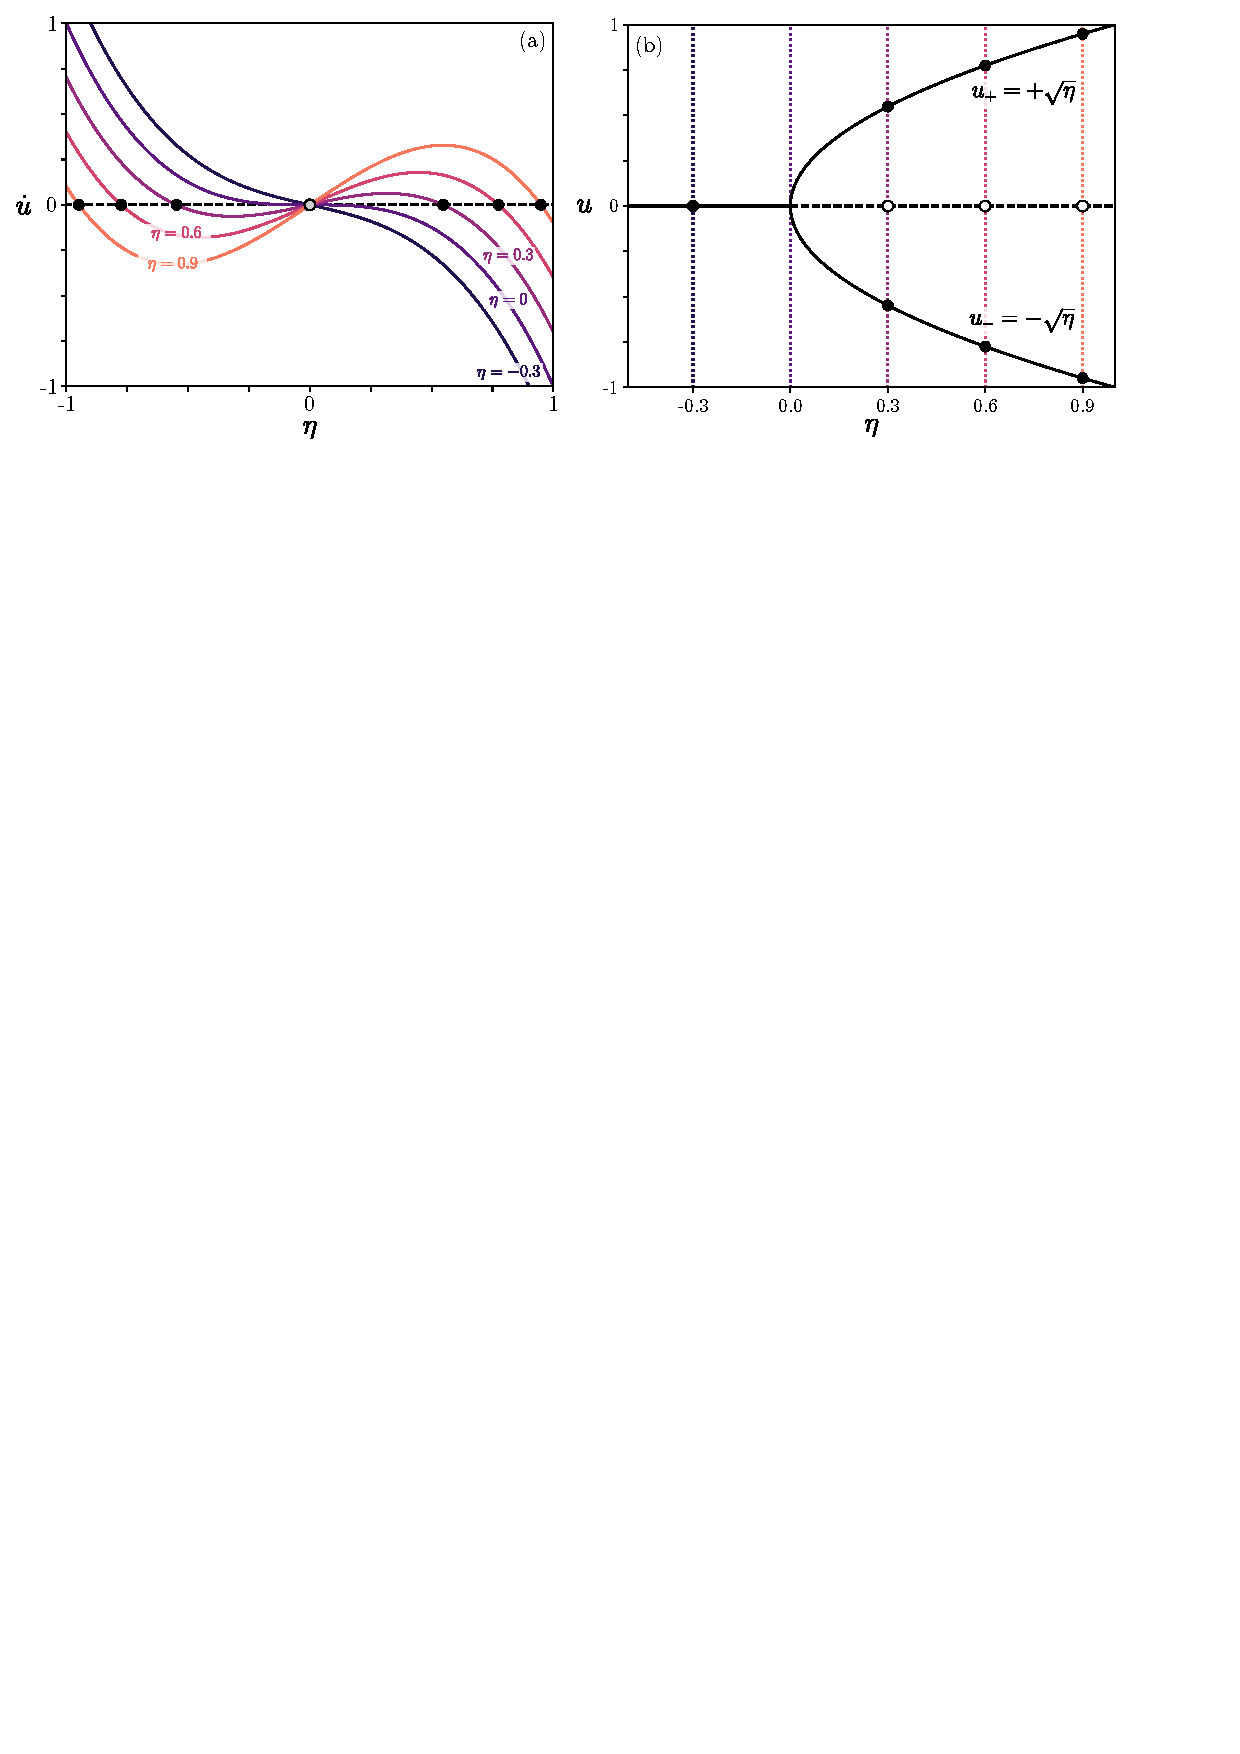
\includegraphics[width=\textwidth]{imagenes/framework/bif_pitch_f.pdf}
    \caption{Prototipical scenario for a pitchfork bifurcation. (a) Phase space
    showing both stable and unstable fixed points for different values of $\eta$. 
    Black circles represent stable fixed points, the grey circle represents a stable for $\eta < 0$
    and unstable for $\eta > 0$ fixed point. (b) Bifurcation diagram showing
    the emergence of two stable branches at the bifurcation, along with the change of
    stability of the trivial solution. Solid (dashed) lines represent
    stable (unstable) branches.}
    \label{fig:pre_bif_pitchfork}
\end{figure}

Two types of pitchfork bifurcations should be distinguished: the {\em supercritical} 
and the {\em subcritical} case. The former corresponds to Eq.~(\ref{eq:pre_bif_pitchfork})
and was discussed above. In the latter, the two symmetric branches that emerge at the bifurcation
point are unstable. In that case, the cubic term in the normal form has a positive sign and
a negative quintic term is added to ensure the solution is bounded, and thus, that is physically
relevant. The modified normal form corresponds to Eq.~(\ref{eq:pre_bif_pitchfork_subcritical}).

\begin{equation}
    \dfrac{du}{dt} = \eta u + u ^ 3 - u^5
    \label{eq:pre_bif_pitchfork_subcritical}
\end{equation}

Moreover, due to the additional quintic term, the symmetric branches are stabilized 
at a secondary saddle-node bifurcation point $\eta_{sn}$, as shown
in Fig.~\ref{fig:pre_bif_subpitchfork}. It is important to mention that in subcritical
bifurcation, a hysteresis loop is typically observed. 
%For instance, Fig.~\ref{fig:pre_bif_subpitchfork}

\begin{figure}[h]
    \centering
    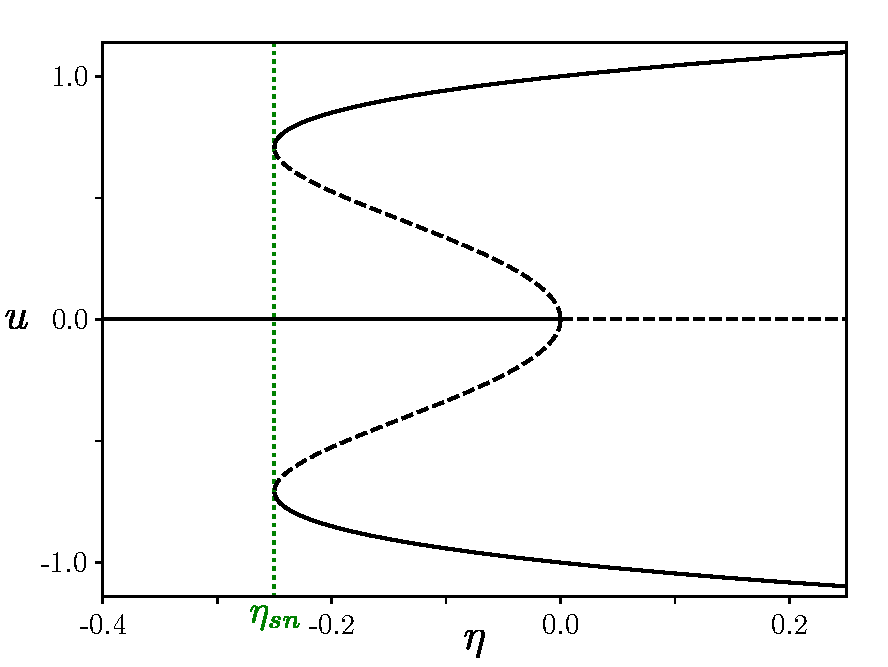
\includegraphics[width=0.6\textwidth]{imagenes/framework/bif_pitch_subcritical.pdf}
    \caption{Bifurcation diagram for the subcritical pitchfork. At the bifurcation point
    for $\eta=0$, two symmetric unstable branches emerge and gain stability after undergoing
    a saddle-node bifurcation for $\eta=\eta_{sn}=-\frac14$. The trivial solution is stable for $\eta < 0$
    and unstable for $\eta > 0$.}
    \label{fig:pre_bif_subpitchfork}
\end{figure}


\subsection{Andronov-Hopf bifurcation}

The two bifurcations discussed previously describe the emergence of steady states or fixed points. 
More specifically, they belong to the class of {\em stationary} bifurcations. Here, a different class of bifurcations will be introduced,
that of {\em dynamical} bifurcations, in which dynamical equilibria emerge. The simplest scenario is the Andronov-Hopf bifurcation
that allows for the emergence of a limit cycle or, in other words, a periodic equilibrium. [Insert examples]. Since oscillations are impossible in 
one dimension [ref strogatz], this bifurcation can only be present in systems of two or more dimensions. For simplicity, the following
analysis will be restricted to only two dimensions. Nevertheless, it can easily be extended to the more general case of arbitrary dimensions.
The normal form can be written in a compact form as a complex equation, Eq.~(\ref{eq:hopf}), for the
order parameter $A = x +iy$. It is important to mention that
the coefficient accompanying the cubic term could be complex, in that case, it corresponds to the Stuart-Landau equation which
is the homogeneous part of the widely known Complex Ginzgurg-Landau equation.

\begin{equation}
    \dfrac{dA}{dt} = (\eta + i\omega)A - |A|^2 A
     \label{eq:hopf}
\end{equation}

It can directly be observed that there is a trivial fixed point at $A=0$. Linear stability analysis around this fixed point 
reveals a pair of complex eigenvalues $\lambda_\pm = \eta \pm i\omega$. Therefore, for $\eta < 0$ the fixed point is a stable
focus, whereas for $\eta > 0$, the eigenvalues have crossed the imaginary axis rendering the focus unstable. Moreover,
by rewriting Eq.~(\ref{eq:hopf}) in polar coordinates $A = re^{i\theta}$, the emergence of a limit cycle is evidenced.

\begin{align}
    \dot{r} &= r(\eta - r^2)\\
    \dot{\theta} &= \omega
    \label{eq:hopf_polar}
\end{align}

From Eq.~(\ref{eq:hopf_polar}) it can be observed that a limit cycle emerges from $\eta=0$ with frequency $\omega$ and an 
amplitude $|A| = r = \sqrt{\eta}$ that increases continuously from zero. 
Similarly, as in the pitchfork bifurcation, this case corresponds to a supercritical
bifurcation given that the limit cycle arising from the bifurcation is stable. Furthermore, the two results mentioned previously
apply also in general, namely, that close to the
bifurcation point $\eta_c$, the amplitude of the limit cycle grows with $\sqrt{\eta - \eta_c}$ and the frequency is approximately
the imaginary part of the eigenvalue at the bifurcation point: $\operatorname{Im}{\lambda(\eta_c)}$.


\begin{figure}[h]
    \centering
    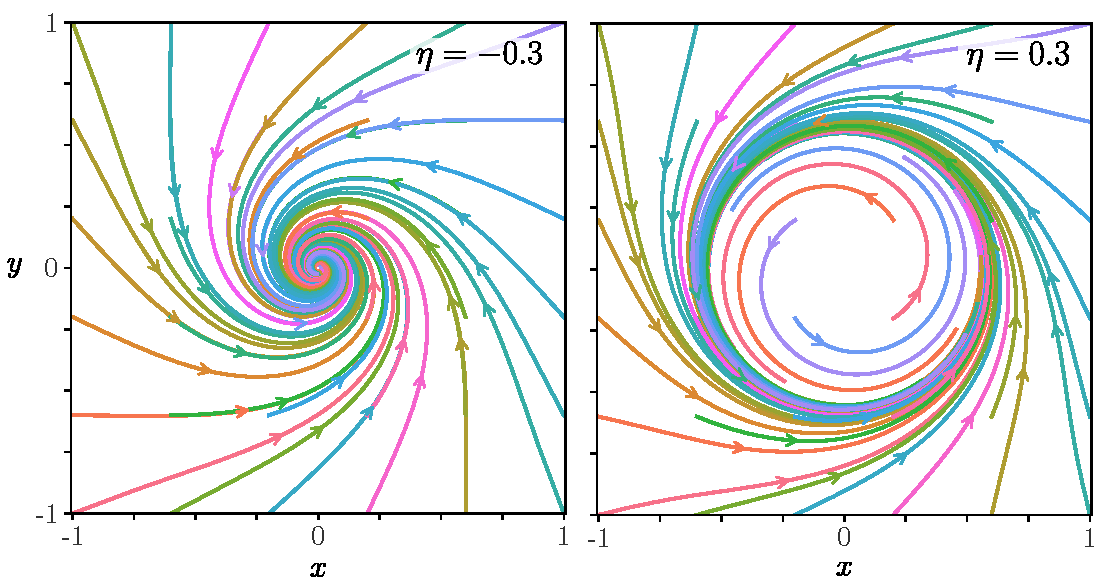
\includegraphics[width=0.8\textwidth]{imagenes/framework/hopf_phasespace.pdf}
    \caption{Phase plane trajectories of Eq.~(\ref{eq:hopf}) showing a stable
    focus for $\eta = -0.3$ in the left panel and a stable limit cycle for $\eta=0.3$
    in the right panel}
\end{figure}

There is, however, a subcritical variation
of the Andronov-Hopf bifurcation in which the emerging limit cycle is unstable and may stabilize at a secondary bifurcation point.
The normal form is similar to the subcritical pitchfork since the cubic term has now the opposite sign and a quintic term is added to ensure the solution is bounded.
Due to the additional quintic term, the emerging limit cycle stabilizes at $\eta_{sn} = -\frac14$ through
a saddle-node bifurcation.

\begin{equation}
    \dfrac{dA}{dt} = (\eta + i\omega) A + |A|^2 A - |A|^4A
\end{equation}

\begin{figure}[h]
    \centering
    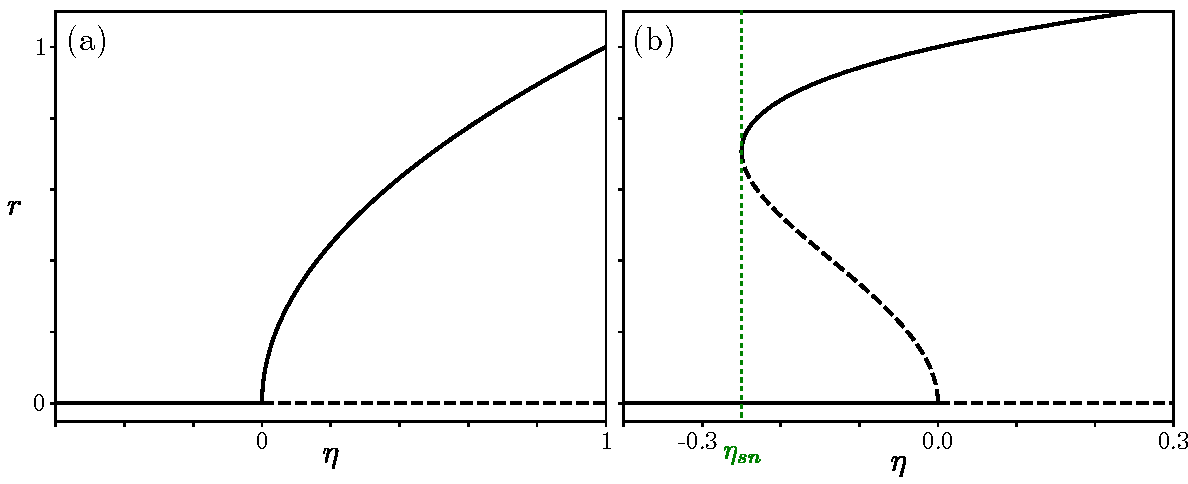
\includegraphics[width=0.9\textwidth]{imagenes/framework/hopf_supersub.pdf}
    \caption{The subcritical and supercritical scenarios of the Andornov-Hopf
    bifurcation. Panel (a) shows the supercritical case and panel (b) shows the subcritical
    case.}
\end{figure}

\section{Localized Structures}
\label{sec:fra_LS}

% In the previous section, the simplest mechanisms for the emergence and
% change of stability of solutions have been discussed, yet little attention
% has been devoted to the solutions themselves. Indeed, in nonlinear dynamical
% systems, an enormous variety of equilibria are possible. In this section,
% special attention will be paid to one particular kind class of equilibria,
% the so-called localized structures. 

Almost a century ago, our understanding of elementary or quantum particles went
through a complete change of paradigm. Indeed, what was originally thought
to be a microscopic speck of matter with a well-defined position, velocity and size
was discovered instead to be a localized wave function lacking the former quantities.
Half a century later, this change of paradigm carried over to meso- and macroscopical out-of-equilibrium
systems. Nicols and Prigogine [insert ref] argued that the energy transfer present in these systems
allows for complex and stable structures to form, such as localized structures. These localized states
or particle-like solutions are supported by a robust balance between gains and losses and have been observed in a
variety of systems due to their universality. 

\begin{figure}[h]
    \centering
    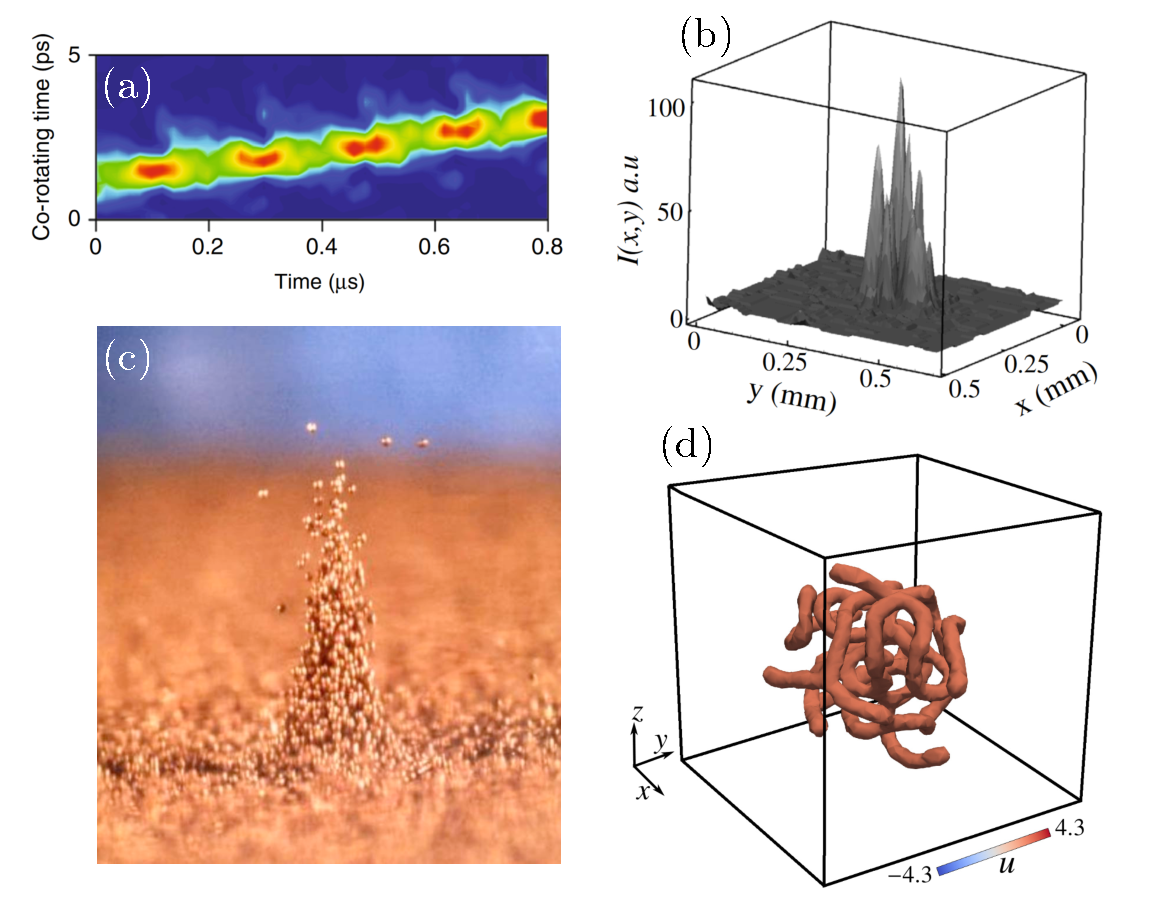
\includegraphics[width=0.7\textwidth]{imagenes/framework/LS/examples_ls.pdf}
    \caption{Examples of localized structures in nonlinear optics, granular media and a simple
    model for pattern formation. Panels (a)-(c) show experimental observations of a drifting breather
    soliton in a microcavity \cite{yi2018imaging}, a chaoticon in a liquid crystal light valve \cite{verschueren2013spatiotemporal}, and an oscillon in a vibrating
    layer of sand \cite{umbanhowar1996localized,aranson2006patterns}. Panel (d) shows a simulation of a localized labyrinth
    in a simple pattern forming model \cite{clerc2021localised, clerc2022localized}.}
    \label{fig:pre_ls_examplesls}
\end{figure}

[Replace by light bullet]

Formally speaking, a LS corresponds to a well localized deviation of some reference background,
typically a homogeneous steady state, although it might also be periodic (in space) or oscillatory (in time).
As illustrated in Figure~(\ref{fig:pre_ls_examplesls}), they have been observed experimentally in one and two spatial dimensions, and predicted numerically in three dimensions.
Their temporal dynamics are quite rich as well, they can present uniform motion, breathing or even chaotic behavior.
From a mathematical point of view, their description relies on partial differential equations or,
in the case of non-local systems, integro-differential equations. At least in one spatial dimension,
it is possible to think of LS as a homoclinic orbit asymptotically approaching the reference state
at the boundaries and performing an excursion in the neighborhood of another equilibrium in the center.
In the more general case of two and three-dimensional LSs, the picture becomes more complex but the
coexistence between two distinct equilibria remains necessary for the formation of LSs.

Willyford Columbo


\subsection{Solitons}

Among localized states, a particularly interesting type are solitons. They were discovered
 for the first time in 1834 by John Scott Russell. He described them 
 as a {\em "large solitary [...] heap of water, which continued its course along the channel without change of form
or diminution of speed"} \cite{russell1845report}. These solitary waves were highly controversial
at the time until Korteweg and de Vries provided an integrable model for shallow water waves
and proved their existence in the now called Korteweg de Vries (KdV) equation \cite{korteweg1895xli}.
It was only a century later that the term soliton was coined by Zabusky and Kruskal
to emphasize their particle-like behavior after observing that solitons in the KdV equation could pass through each
other with no change in shape or speed \cite{zabusky1965interaction}. In the following
years, the newly discovered inverse scattering transform \cite{gardner1967method, gardner1974korteweg}
allowed to completely solve the KdV equation and find the analytical expression of solitons.
Immediately after, it was extended to other integrable and conservative equations such as the nonlinear Schrödinger (NLS)
equation \cite{shabat1972exact} and the sine-Gordon equation \cite{ablowitz1973method}. 
In these systems, they arise due to a balance between dispersion and nonlinearity. 


More recently, the term dissipative soliton (DS) was introduced to extend the previous definition
and refers to a qualitatively
similar state, but in driven dissipative systems, where there is a continuous energy influx and 
dissipation, requiring thus a balance between influx and dissipation. 
Although there is not a commonly agreed-upon definition of DSs, they typically
exhibit certain features. Firstly, DSs are attractors with well-defined amplitude and shape, and
possess a characteristic length independent of the system size or boundary. Moreover, they
tend to interact with other nearby DSs in a manner reminiscent of classical particles. 
As a result, they often receive the name of particle-like states. It is important to emphasize that classical (conservative) solitons and dissipative solitons
are two very different structures; the mathematics behind their presence, and therefore their
properties, are distinct.

In the following sections, a more in-depth description of LSs and DSs will be presented 
in the context of two paradigmatic models: the Swift-Hohenberg equation and the Lugiato-Lefever
equation.  


\subsection{Turing-Swift-Hohenberg equation}

The Turing-Swift-Hohenberg equation is possibly the simplest and most studied model 
for the formation of patterns and localized structures, see \cite{cross1993pattern,knobloch2015spatial}
for a comprehensive review. It was first introduced
by Swift and Hohenberg as a phenomenological model to describe Rayleigh-Bénard
convection \cite{swift1977hydrodynamic,pomeau1979stability}, although it was later 
known that Turing had already written 
a similar and more general equation in the context of morphogenesis \cite{dawes2016after}.
The TSHE can be written in several forms, depending on the nonlinearities. The most common
presents only a cubic nonlinearity, similar to a supercritical pitchfork; while other
variations with either a quadratic-cubic or cubic-quintic nonlinearities can be envisaged \cite{knobloch2015spatial}.
In the former case, the pattern (spatially periodic) state emerges supercritically whereas in the latter,
it emerges subcritically. Since a coexistence between the pattern and the trivial state is necessary for the formation of LSs,
the subcritical case will be the focus of the following discussion, and in particular the case of 
the cubic-quintic TSHE,

\begin{equation}
    \partial_t u = \varepsilon u + u ^3 - u^5 - \nu \nabla^2 u - \nabla^4 u,
    \label{eq:pre_ls_she}
\end{equation}

where $u$ is a real scalar field, $\varepsilon$ is the control parameter and $\nu>0$ can be set to
one without loss of generality. It can be noted that Eq.~(\ref{eq:pre_ls_she}) is reflection symmetric
with respect to both the $x$ and $u$ axes, i.e. is invariant under transformation $x\to -x$ and $u\to -u$.
Moreover, the equation is variational, meaning that it minimizes a Lyapunov (or free energy) functional
$\mathcal{F}[u]$ such that,

\begin{equation}
    \mathcal{F} = \dfrac12 \int_{-\infty}^{\infty} -\varepsilon u^2 - \dfrac12 u^4 + \dfrac13 u^6 - (\nabla u)^2 + (\nabla^2 u)^2 \ d^dr.
\end{equation}

As a result, the solutions of Eq.~(\ref{eq:pre_ls_she}) are stationary.
In principle, Eq.~(\ref{eq:pre_ls_she}) can be written in 
$d$ spatial dimensions, however, the following discussion will be restricted to the case of $d=1$ for simplicity.
It can be observed that the TSHE admits a trivial solution $u=0$. Linear
stability analysis with respect to perturbations of the form $\delta u = e^{\sigma t + ikx}$ yields
the following dispersion relation for the growth rate,

\begin{equation}
    \sigma = \varepsilon + \nu k^2 - k^4.
    \label{eq:pre_ls_she_disp}
\end{equation}

The critical mode for which patterns emerge can be obtained by setting $\sigma = 0$ in Eq.~(\ref{eq:pre_ls_she_disp}),
revealing the critical wavenumber $k_c^2 = \frac{\nu}{2} \pm \sqrt{\varepsilon - \frac{\nu^2}{4}}$. From where
it can be inferred that patterns emerge at a critical point (also called Turing point, or modulational instability) 
$\varepsilon_c = \frac{\nu^2}{4}$. For increasing values of $\varepsilon$,
the critical mode along with its neighboring band of modes become unstable, leading to an exponential growth
until it saturates due to the nonlinear terms. As a result, patterns form with a characteristic length scale determined
by $k_c$ (at least in the absence of boundaries).

Furthermore, perturbation theory close to the bifurcation point \cite{burke2007snakes}
predicts that the pattern state emerges subcritically, along with four branches of
localized states parametrized by their phase $\phi = 0, \pi/2, \pi, 3\pi/2$. These
four branches come in even ($\phi = 0, \pi$) and odd ($\phi = \pi/2, 3\pi/2$) pairs.
Each pair of branches is related by a reflection symmetry $u \to -u$, and thus,
share the same norm. By means of numerical continuation (see Chapter~\ref{ch:continuation}),
the solution branches far from the bifurcation point can be followed, revealing the
bifurcation diagram shown in Fig.~(\ref{fig:pre_ls_she_bif}).

\begin{figure}[h]
    \centering
    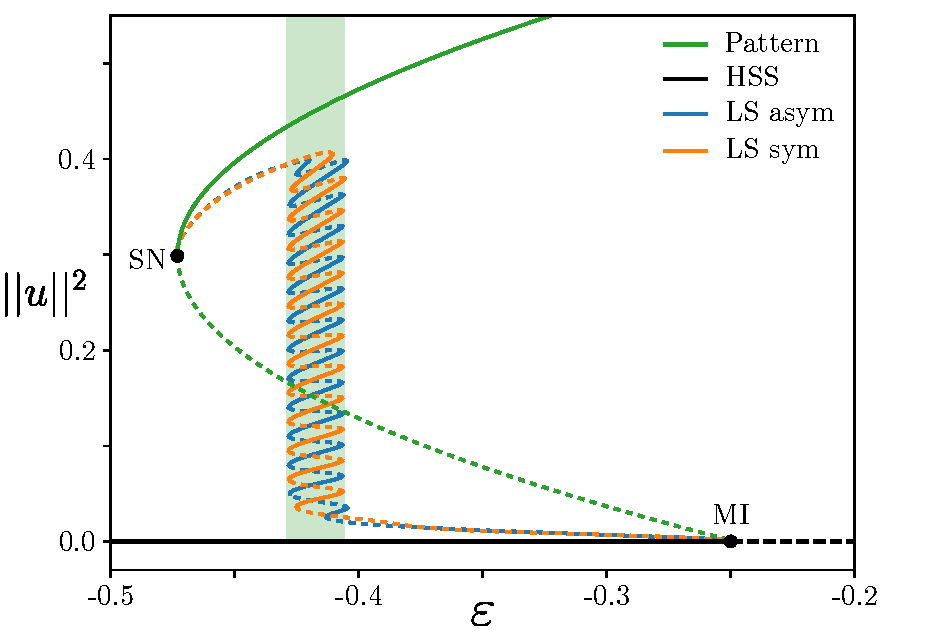
\includegraphics[width=0.7\textwidth]{imagenes/framework/LS/snaking_she35.pdf}
    \caption{Bifurcation diagram showing the two pairs of symmetric (blue) and asymmetric
    (orange) localized states, along with the homogeneous steady state (black) and the pattern state (green).
    Solid (dashed) lines represent stable (unstable) branches.}
    \label{fig:pre_ls_she_bif}
\end{figure}

An intriguing feature of Eq.~(\ref{eq:pre_ls_she}) is the snaking behavior of the branches of LSs, as shown
in Fig.~(\ref{fig:pre_ls_she_bif}). More specifically, it can be observed that a new wavelength 
is added to the LSs after undergoing a pair of saddle-node bifurcations.
This so-called homoclinic snaking is a consequence of the heteroclinic entanglement
between the stable and unstable manifolds of the HSS and pattern state, 
respectively~\cite{woods1999heteroclinic,coullet2000stable}.

\begin{itemize}
    \item Turing-Swift-Hohenberg as a paradigmatic and simple equation for pattern
formation. History. Read review from Hohenberg.
    \item Physical description, relevance to physical systems experiments. 
    Rayleigh-Benard convection? Buckling of a cylinder? Main results, vegetation,
    pattern formation on a disk Verschueren
    \item Mathematical motivation 1, pattern formation, critical modes etc
    \item Mathematical motivation, why is it simple why does it allow for LS.
Reversibility, hyperbolic points allow for a homoclinic connection
    \item Homoclinic snaking, manifolds etc.
\end{itemize}

\subsection{Spontaneous symmetry breaking and motion instabilities}

\begin{itemize}
    \item Motion fundamental, ubiquitous in this dissertation! Asymmetry behind motion.
    \item Forced symmetry breaking? (spectral filtering, raman, etc)
    \item Symmetric systems? Spontaneous symmetry breaking
\end{itemize}

Article by Alejandro Alvarez and references therein.


\subsection{Resonant cavities and the Lugiato-Lefever equation}

\begin{itemize}
    \item Optics and nonlinear phenomena, dissipative structures / localized structures in otpics?
    \item Lugiato-Lefever as a simple nonlinear model for resonant cavities that allows for the
    formation of dissipative structures, similar to Prigogine
    \item Main results, very good agreement theory/experiment, mention main experiments.
    applications with combs.
    \item Mathematical analysis, normal/anomalous regime, MI, etc.
\end{itemize}

[normal, anomalous regime, MI etc]

\subsection{Non-local effects in the LLE}

\begin{itemize}
    \item Dispersion curve, HOD
    \item Memory effects, scattering
    \item Experimental elements, spectral filtering
\end{itemize}

\subsubsection{Raman effect}
\subsubsection{Spectral filtering}

\section{Phase oscillators and Chimera states}
Connection to LS?  Revisit chapter
\subsection{Phase oscillators}
\label{sec:phase_oscillators}

\subsection{Kuramoto model}

\subsection{Chimera states}

\subsection{Ott-Antonsen manifold reduction}